\projecthead{08 / Analysis}{Hydrogen engine study}{Comparative performance \& operating constraints}{June 2024}
\textit{Comparative study}
\par\medskip An investigation of electrolysis-derived hydrogen in an internal combustion engine, comparing performance and operating demands with gasoline.
\par\smallskip {\small\color{muted} Tools: Research, Python, data analysis}
\medskip
\noindent
\begin{minipage}[t]{.48\linewidth}\centering\vspace{0pt}

\includegraphics[width=\linewidth,height=1.8in,keepaspectratio]{images/hydrogen/engine-test-setup.png}
\par\smallskip{\footnotesize\color{muted} Hydrogen engine experiment: gas-generation apparatus, tubing, and engine.}\end{minipage}\hfill
\begin{minipage}[t]{.48\linewidth}\centering\vspace{0pt}
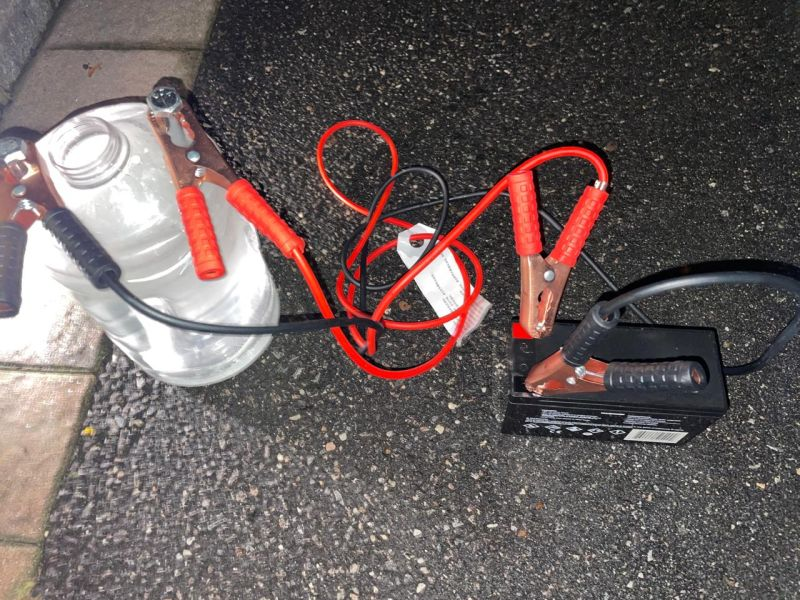
\includegraphics[width=\linewidth,height=1.8in,keepaspectratio]{images/hydrogen/electrolysis-power-setup.png}
\par\smallskip{\footnotesize\color{muted} Gas-generation apparatus connected to the battery supply.}\end{minipage}\hfill
\par\medskip
\subsection*{Research question}
Compared engine behavior and operating overhead for hydrogen and gasoline, focusing on efficiency, speed, and thermal demands.
\subsection*{Reported observations}
The study reported 40\% higher RPM and 60\% higher operating temperature for the hydrogen-fueled engine relative to the gasoline baseline. The thermal result motivated closer attention to material constraints.
\subsection*{Design implication}
The temperature result highlights thermal management and material constraints as priorities for subsequent investigation.